\section{Evaluation}
\label{sec:results}

This section evaluates whether off-the-shelf LLMs can act as useful Roofline triage tools for GPU kernels, organized around the four research questions of \autoref{sec:introduction}.

Unless stated otherwise, the cross-model comparisons use the 732-sample shared subset of \autoref{sec:task-methodology}.
We report nonzero \bandwidthbound/\computebound regime classification as the primary outcome and treat the numeric \rai error as a diagnostic that explains \textit{why} a classification succeeds or fails.
Because the \rai-percent-error distributions are heavy-tailed, we emphasize balanced accuracy, medians, and interquartile behavior rather than means.
In the tables that follow, we abbreviate the two evidence settings as SO (\sourceonly) and S+S (\sourcesass).






\subsection{RQ1: Can LLMs Classify the Roofline Regime From Static Artifacts?}

For FP32 and FP64, yes; for FP16, not from \sourceonly evidence.
\autoref{tab:compute-bound-prf} reports nonzero \bandwidthbound/\computebound balanced accuracy by model, precision, and evidence setting.
There are a few trends to note:
\textbf{(1)} From \sourceonly prompts, \opus classifies the FP32 regime at 0.940 balanced accuracy and FP64 at 0.755; \gptfivefour reaches 0.889/0.670, and even the budget \gptoss reaches 0.875/0.690.
These are strong numbers for a pre-compilation signal: the models recover the compute-versus-memory branch for most FP32 and FP64 kernels using only source code, build context, runtime arguments, and GPU specifications.
\textbf{(2)} The FP16 case is a clean failure.
From \sourceonly prompts, every model---including the frontier ones---sits exactly at the 0.500 chance baseline for FP16.
The same models that classify FP32 and FP64 regimes well are no better than a coin flip on FP16 under \sourceonly evidence; we return to why in RQ2.

Because the panel is \computebound-poor (\autoref{sec:task-methodology}), we confirm the strong numbers are not an over-prediction artifact: the \computebound precision/recall breakdown (\autoref{tab:compute-bound-prf}) shows \sourceonly \opus reaches 1.000 \computebound precision at 0.880 recall for FP32, and 0.966 precision at 0.528 recall for FP64.
The lower FP64 recall is honest---the models miss roughly half of the compute-bound FP64 kernels even when they place the rest correctly.

The takeaway is that \textbf{(a)} off-the-shelf LLMs are already reliable FP32 and FP64 regime classifiers from \sourceonly artifacts, with a clear ``you-get-what-you-paid-for'' ordering from \gptoss to \opus, and \textbf{(b)} FP16 triage is not available from \sourceonly evidence and must escalate to more evidence, which motivates RQ2.

\begin{rqsummary}
\textbf{RQ1 Summary:} From \sourceonly artifacts, off-the-shelf LLMs reliably classify the FP32 and FP64 Roofline regimes---\opus reaches 0.940 balanced accuracy on FP32 and even the budget \gptoss reaches 0.875---but under the same \sourceonly evidence every model, frontier ones included, is no better than a coin flip on FP16.
\end{rqsummary}






\subsection{RQ2: What Does Cross-Compiled SASS Add, and Why?}

It closes the FP16 gap, and the mechanism is compiler-synthesized arithmetic.
Adding \sourcesass lifts FP16 \bandwidthbound/\computebound balanced accuracy from the 0.500 \sourceonly baseline to 0.984 for \opus and 0.870 for \gptfivefour (\autoref{tab:compute-bound-prf}).
The gain is specific to the evidence, not the model: the same frontier models were at chance for FP16 under \sourceonly, while \gptoss---which makes weaker use of long SASS prompts---only reaches 0.583.
\sourcesass helps FP32 and FP64 much more modestly (\opus FP32 balanced accuracy rises 0.940$\rightarrow$0.967, FP64 0.755$\rightarrow$0.765), because FP32 and FP64 arithmetic is already mostly source-visible.

The reason is mechanistic and visible in the collected samples.
FP16 throughput on these GPUs comes from packed \texttt{HFMA2} instructions that the compiler synthesizes; they are not syntactically present in source, so \sourceonly reasoning conservatively predicts zero FP16 work.
%In the \texttt{accuracy-cuda} kernel on the A100, \sourceonly \opus predicts zero FP16 work and gets the regime wrong, while under \sourcesass it attributes the nonzero FP16 signal to an executed \texttt{HFMA2.MMA} instruction and classifies correctly.
This is why the result generalizes beyond a single model: \textit{FP16 Roofline reasoning requires compilation, not execution}, and cross-compilation supplies it without access to the target GPU.

\noindent\textbf{Numeric \rai as a diagnostic.}
The numeric error tracks the same evidence boundary, which is why we read it as a diagnostic rather than a headline.
\autoref{fig:nonzero-ape} shows the distribution of nonzero \rai absolute percent error.
Where classification is strong the numeric estimate is also close: under \sourcesass, \opus lands within 25\% error of the profiled \rai on 47.0\% of nonzero FP16, 53.0\% of FP32, and 44.0\% of FP64 samples, with median errors of 20.4\%, 18.3\%, and 15.3\%.
Where \sourceonly is blind (FP16), numeric accuracy collapses to under 1\% of samples within 25\%.
The distributions are heavy-tailed (i.e. some kernels are predicted almost exactly while others are orders of magnitude off) so a deployed tool should treat numeric \rai as a coarse hint and rely on the more robust regime classification.

\begin{figure}[t]
  \centering
  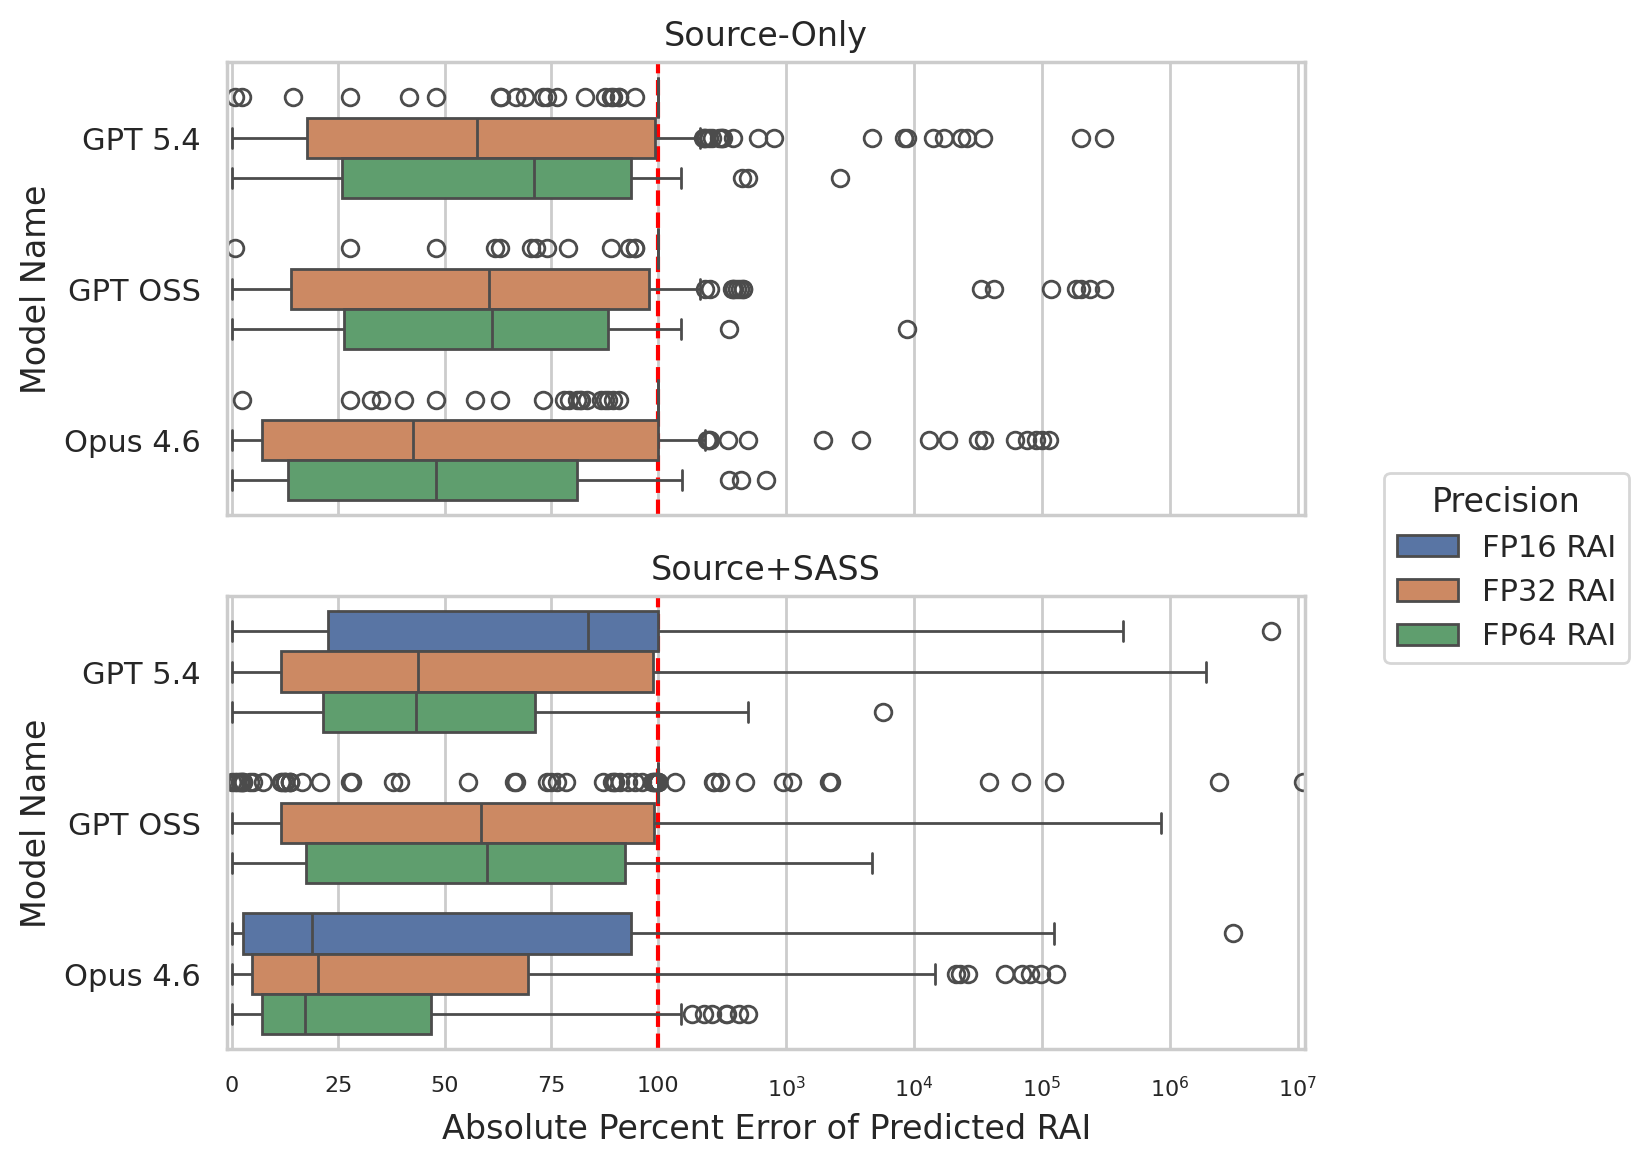
\includegraphics[width=\linewidth]{figures/nonzero_ape_boxplots.png}
  \caption{Absolute percent error on nonzero \rai cases, by model, precision, and evidence setting.
  The distribution has both a useful low-error region and a long failure tail.
  \sourcesass sharply expands the low-error FP16 region for the frontier models and tightens many FP32/FP64 distributions, mirroring the classification gains.}
  \label{fig:nonzero-ape}
\end{figure}

\noindent\textbf{Error-prone code features.}
\begin{table}[t]
  \centering
  \caption{Cliff's $\delta$ between feature-present and feature-absent nonzero \rai error distributions (SO~=~\sourceonly, S+S~=~\sourcesass). Positive $\Rightarrow$ higher error when the feature is present.}
  \label{tab:feature-error-association}
  \scriptsize
  \setlength{\tabcolsep}{4pt}
  \resizebox{\columnwidth}{!}{%
  \begin{tabular}{l rr rr rr}
    & \multicolumn{2}{c}{\gptfivefour} & \multicolumn{2}{c}{\gptoss} & \multicolumn{2}{c}{\opus} \\
    \cmidrule(lr){2-3}\cmidrule(lr){4-5}\cmidrule(lr){6-7}
    Feature & SO & S+S & SO & S+S & SO & S+S \\
    \midrule
    Has FLOP Division        & 0.32 & 0.34 & 0.33 & 0.34 & 0.34 & 0.36 \\
    Has Float Subexprs       & 0.30 & 0.32 & 0.29 & 0.32 & 0.30 & 0.31 \\
    Has Special Math         & 0.26 & 0.26 & 0.25 & 0.28 & 0.25 & 0.29 \\
    Has Loop-Invariant FLOPs & 0.24 & 0.27 & 0.22 & 0.21 & 0.23 & 0.27 \\
    \midrule
    Calls Helper Function     & 0.11 & 0.14 & 0.10 & 0.15 & 0.15 & 0.15 \\
    Has RNG Inputs            & 0.11 & 0.12 & 0.11 & 0.13 & 0.12 & 0.14 \\
    Has Branching             & 0.08 & 0.09 & 0.11 & 0.11 & 0.10 & 0.09 \\
    Uses Preproc Defines      & 0.06 & 0.08 & 0.07 & 0.06 & 0.08 & 0.09 \\
    Has Data-Dep Branching    & 0.07 & 0.07 & 0.04 & 0.06 & 0.07 & 0.08 \\
    Uses Input Data from File & 0.02 & 0.01 & 0.05 & 0.04 & 0.02 & 0.01 \\
    Deterministic Grid Size   & 0.01 & 0.01 & 0.01 & 0.01 & 0.03 & 0.02 \\
    Deterministic Block Size  & $-0.04$ & $-0.03$ & $-0.08$ & $-0.09$ & $-0.07$ & $-0.04$ \\
  \end{tabular}%
  }
\end{table}

Using the source-feature labels of \autoref{sec:task-methodology}, the residual numeric errors concentrate where the same code patterns appear regardless of model or prompt type (\autoref{tab:feature-error-association}).
Four FLOP-perturbing features dominate across every model and evidence setting---FLOP division, reusable float subexpressions, transcendental (``special'') math functions, and loop-invariant FLOP work, each with a Cliff's $\delta$ around 0.2--0.36---whereas structural features such as deterministic launch bounds show essentially no association.
These features either inject FLOPs the compiler lowers from a single source token (division, transcendentals) or remove repeated work the model over-counts statically (subexpression elimination, loop-invariant hoisting), so they directly perturb the FLOP term of \rai.
The practical implication is that users should expect the largest \rai errors---and should most want SASS---on kernels dense in these features.

\begin{rqsummary}
\textbf{RQ2 Summary:} Cross-compiled \sourcesass closes the FP16 gap, lifting FP16 accuracy from 0.500 to 0.984 for \opus, because it exposes the compiler-synthesized packed-half (\texttt{HFMA2}) arithmetic that source hides; FP32 and FP64, already source-visible, gain little.
FP16 Roofline reasoning therefore requires post-compilation evidence for accurate regime classification.
%compilation, not execution---and cross-compilation supplies it without the target GPU.
\end{rqsummary}






\subsection{RQ3: How Consistent Are the Predictions Across Repeated Queries?}

LLM predictions are nondeterministic, so a single query per kernel cannot establish reliability.
We resample the models on the small, stratified panel mentioned in \autoref{sec:study-design} and measure two kinds of consistency: the median coefficient of variation (MCV) of the predicted \rai across repeats, and whether the \bandwidthbound/\computebound prediction is unanimous across repeats (i.e. agreement).
\autoref{tab:repeated-query-variance} reports both metrics.

\begin{table*}[t]
  \centering
  \caption{Repeated-query response variability on the repeat-trials panel. ``CV'' is the median coefficient of variation of predicted \rai across repeats (lower is more consistent); ``Agr'' is the fraction of cells whose \bandwidthbound/\computebound call is unanimous across repeats. Computed at the main-paper decode settings.}
  \label{tab:repeated-query-variance}
  \scriptsize
  \setlength{\tabcolsep}{4pt}
  \begin{tabular}{llrrrrrr}
    \toprule
    & & \multicolumn{2}{c}{FP16} & \multicolumn{2}{c}{FP32} & \multicolumn{2}{c}{FP64} \\
    \cmidrule(lr){3-4}\cmidrule(lr){5-6}\cmidrule(lr){7-8}
    Model & Evidence & CV & Agr & CV & Agr & CV & Agr \\
    \midrule
    \texttt{GPT OSS} & source-only & 0.00 & 100\% & 0.27 & 81\% & 0.20 & 76\% \\
    \texttt{GPT OSS} & source+SASS & 0.00 & 95\% & 0.44 & 69\% & 0.49 & 62\% \\
    \bottomrule
  \end{tabular}
\end{table*}


Three trends stand out.
\textbf{(1)} The decision-level prediction is generally stable: it is unanimous across repeats for most kernels, with per-configuration agreement mostly in the 82--100\% range, so the headline classification is not an artifact of a single lucky draw.
\textbf{(2)} The most accurate model is also the most consistent.
\opus holds a near-zero MCV and 88--100\% agreement in \emph{both} evidence settings, and, unlike the other models, adding SASS barely perturbs it (FP16 MCV stays 0.00 at 96\% agreement).
The model one would actually deploy is therefore also the most reliable, and for \opus single-shot use is comparatively safe.
\textbf{(3)} Where SASS does destabilize predictions, the effect is model-specific rather than intrinsic to the evidence: \gptfivefour's MCV jumps from essentially zero under \sourceonly to 0.87 (FP16), 0.61 (FP32), and 0.33 (FP64) once SASS is added, and \gptoss's \sourcesass agreement falls to 69\% for FP32 and FP64.
This is the cost of the evidence that cracks FP16 for the weaker models: once a model commits to a numeric FP16 estimate rather than a degenerate zero, that estimate varies more across repeats.

\begin{rqsummary}
\textbf{RQ3 Summary:} Decision-level predictions are mostly stable (82--100\% agreement across repeats). \opus is both the most accurate and the most consistent, so a single query usually suffices; the cheaper models and \gptfivefour under \sourcesass vary enough that a deployed tool should issue a few repeated queries and take the majority \bandwidthbound/\computebound vote.
\end{rqsummary}






\subsection{RQ4: How Do the Signals Compare in Accuracy and Cost?}

The LLM signals form a clear cost/accuracy tier, they are inexpensive in absolute per-query terms, and (unlike profiling) they need no target-hardware access.

\noindent\textbf{Cost tiering.}
\autoref{tab:compute-bound-prf} reports median per-query cost, per LLM-evidence configuration.
The budget \gptoss classifies the \sourceonly FP32 regime at 0.875 balanced accuracy for a median \$0.0006 per query; \gptfivefour reaches 0.889 for \$0.0197; and \opus reaches 0.940 for \$0.0679.
For FP16, only the SASS-backed frontier tier works, at \$0.0315 (\gptfivefour) to \$0.1066 (\opus) per query.
The \sourceonly FP32 tier is inexpensive in absolute terms: at a median \$0.0006 per kernel it needs no target-hardware access at all, unlike profiling.
We do not present end-to-end build-and-profile timings, so we make no measured time- or cost-saving claim against profiling; the advantages we establish are absolute query cost and the elimination of target-hardware access.
The frontier+SASS tier that additionally cracks FP16 is the premium option, and its higher per-query cost is the case where directly profiling may be preferable if the target hardware is available.

\noindent\textbf{Versus static baselines.}
\begin{table*}[t]
  \centering
  \caption{Best off-the-shelf LLM versus best static reference for nonzero \bandwidthbound/\computebound triage on the shared subset. Each cell gives BAcc and nonzero MdAPE for the strongest method in that evidence family; discordant-pair columns report exact paired wins on the same samples.}
  \label{tab:llm-vs-static}
  \scriptsize
  \setlength{\tabcolsep}{4pt}
  \begin{tabular}{lllrllr}
    Evidence & Precision & Best LLM & BAcc / MdAPE & Best static & BAcc / MdAPE & Discordant wins LLM/static ($p$) \\
    \midrule
    \sourceonly & FP16 & \gptfivefour & 0.500 / 100.0 & Source learned ET & 0.723 / 217.7 & 10/17 (0.248) \\
    \sourceonly & FP32 & \opus & 0.940 / 43.9 & Source learned RF & 0.750 / 100.0 & 52/3 ($<0.001$) \\
    \sourceonly & FP64 & \opus & 0.755 / 52.0 & Lexical Heuristic & 0.683 / 99.5 & 21/13 (0.229) \\
    \sourcesass & FP16 & \opus & 0.984 / 20.4 & SASS learned ET & 0.608 / 163.1 & 33/5 ($<0.001$) \\
    \sourcesass & FP32 & \opus & 0.967 / 18.3 & SASS learned ET & 0.730 / 100.0 & 57/4 ($<0.001$) \\
    \sourcesass & FP64 & \opus & 0.765 / 15.3 & SASS learned RF & 0.841 / 62.4 & 5/13 (0.096) \\
  \end{tabular}
\end{table*}

To establish that the LLM signal is worth its cost beyond off-the-shelf prompting, \autoref{tab:llm-vs-static} compares the best off-the-shelf LLM against the best static reference---the learned random-forest (RF) and extra-trees (ET) regressors of \autoref{sec:task-methodology}, alongside lightweight lexical heuristics---for nonzero \bandwidthbound/\computebound triage, per precision and evidence setting on the 732-kernel subset.
Because both methods run on the same kernels, we compare them with a paired (McNemar) test: the discordant-wins column counts kernels where exactly one method is correct, reported as LLM wins/static wins, with $p$ testing whether the LLM wins significantly more of these disagreements.
Where the signal matters most the LLMs win decisively and significantly on the same samples: \sourceonly FP32 (\opus 0.940 vs.\ 0.750 balanced accuracy, 52/3 discordant wins), \sourcesass FP16 (0.984 vs.\ 0.608, 33/5), and \sourcesass FP32 (0.967 vs.\ 0.730, 57/4), and in each of these the LLM's numeric \rai error is far lower (MdAPE 18--44\% vs.\ 100--163\%).
The static baselines are competitive only in the two regimes where the LLMs are weakest: \sourceonly FP16, where neither method is usable---the best LLM is degenerate at 0.500 while the best static reaches 0.723 but with a 218\% MdAPE---and \sourcesass FP64 triage, where a learned tree edges \opus on balanced accuracy (0.841 vs.\ 0.765) but not significantly ($p=0.096$) and still with a worse numeric error (62\% vs.\ 15\% MdAPE).
Across the six regimes the LLMs significantly beat the best static baseline in three---the high-value SASS-backed and FP32 frontier regimes---and the remaining differences are not statistically significant; even where a static baseline edges ahead on the classification call, its \rai estimate is too coarse to be used as a numeric diagnostic.

\begin{rqsummary}
\textbf{RQ4 Summary:} In the high-value regimes the LLMs significantly beat lightweight static baselines (e.g.\ \sourcesass FP16 0.984 vs.\ 0.608 balanced accuracy, $p<0.001$), at fractions of a cent per query and with no target-hardware access. No single configuration wins every regime, so the cost-effective choice is to match the model and evidence tier to the target precision.
\end{rqsummary}

The takeaway across the four RQs is that off-the-shelf LLMs are a practical, hardware-free Roofline triage tool once matched to the available evidence: \sourceonly artifacts suffice for FP32 and FP64 at fractions of a cent, cross-compiled SASS is what unlocks FP16, and single-shot use is safe for a frontier \opus model but should become a small majority vote for the cheaper \gptfivefour and \gptoss models.
